\chapter{Resultados preliminares}
\label{cap:results}

\section{Coleta preliminar}

Na coleta preliminar, foram adquiridos vídeos e os sinais correspondentes provenientes de monitores multiparamétricos de três pacientes admitidos na UTI. Em um dos casos, o oxímetro de pulso não estava conectado no momento da aquisição, impossibilitando a obtenção do sinal de fotopletismografia de referência. Entre os dois pacientes restantes, um encontrava-se sob suporte ventilatório mecânico e sedação, enquanto o outro estava em estado ativo e sem suporte ventilatório. A seguir, são expostos os resultados do processamento dos sinais obtidos. 

% L7 - paciente 1
% L9 - paciente 2
% L8 - paciente 3

\subsection{Sincronização de dados}

Para realizar a sincronização dos vídeos com os dados de referência, foi realizada uma análise de correlação baseada no índice de correlação de Pearson entre estimativas de frequência cardíaca realizadas a partir do eletrocardiograma e as estimativas realizadas a partir do sinal de rPPG extraído por cada um dos métodos não supervisionados citados na \autoref{tab:metodos_rppg}, conforme exemplifica a \autoref{fig:sinc-L9}. Com isso, foi obtido o gráfico de correlação média entre todos os métodos para cada paciente, como pode ser observado no exemplo da \autoref{fig:mean-corr-L9}. A partir do ponto de maior correlação em cada caso, foi obtido o intervalo a ser considerado para a extração dos dados de referência. 

\begin{figure}[h!]
    \centering
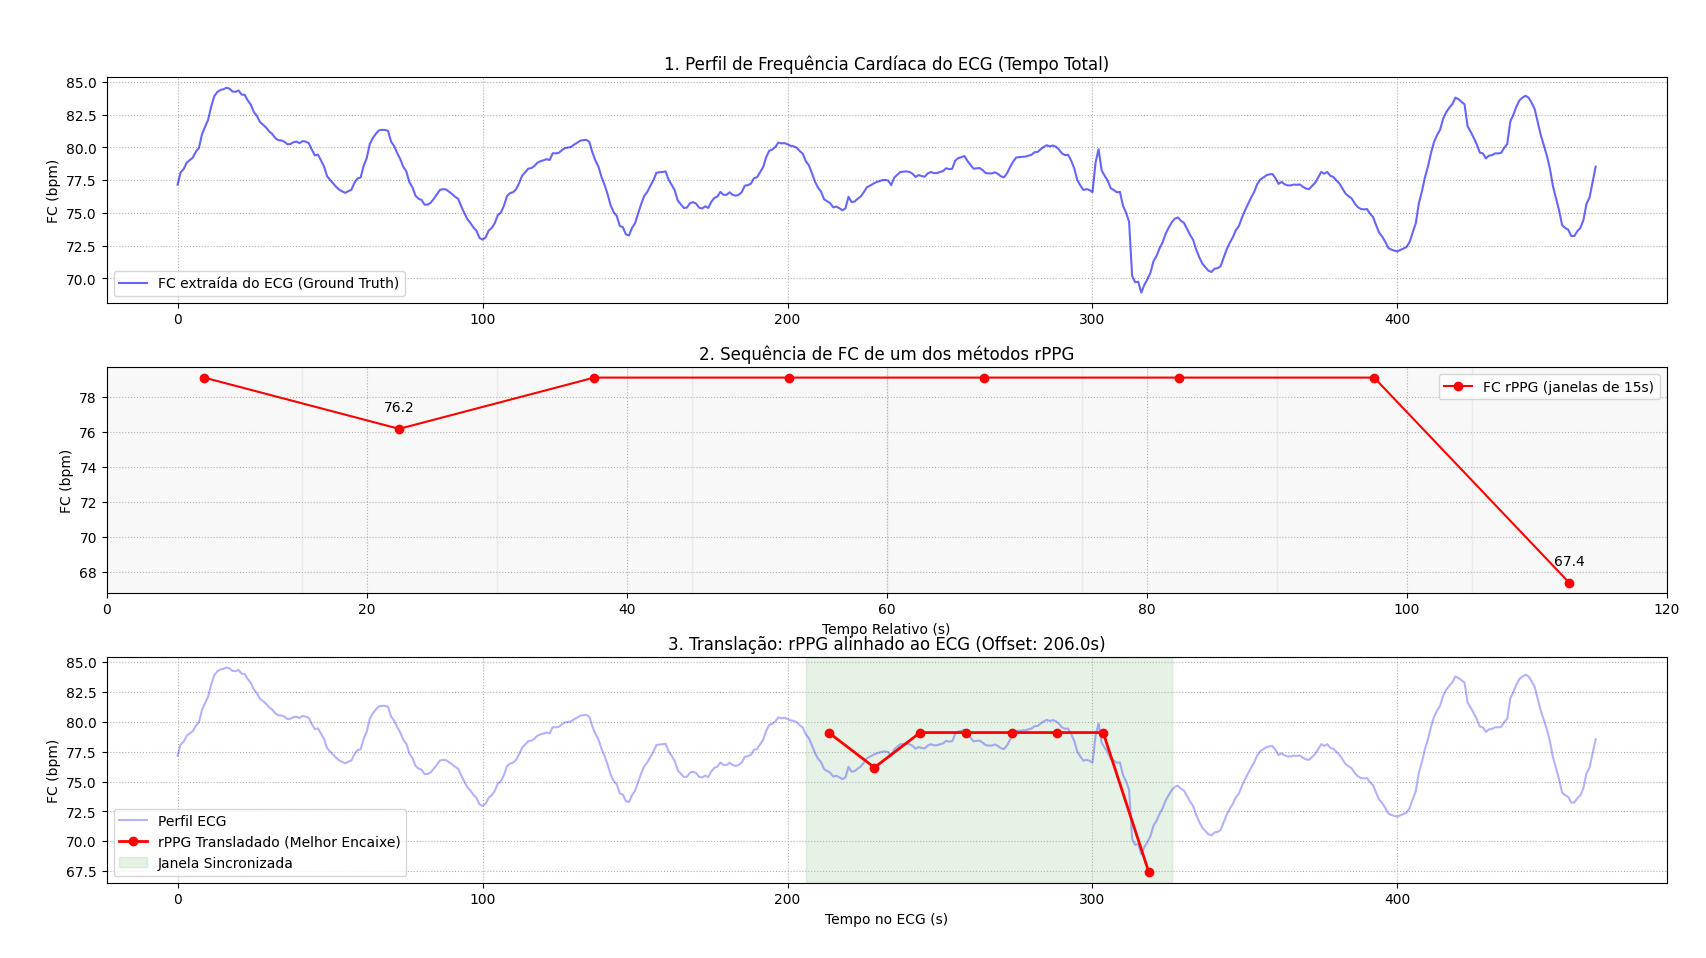
\includegraphics[width=1\linewidth]{imagens/hr_L9.png}
    \caption{Etapas de definição do intervalo considerado para os dados de referência do paciente 2}
    Fonte: autoria própria
    \label{fig:sinc-L9}
\end{figure}

\begin{figure}[h!]
    \centering
        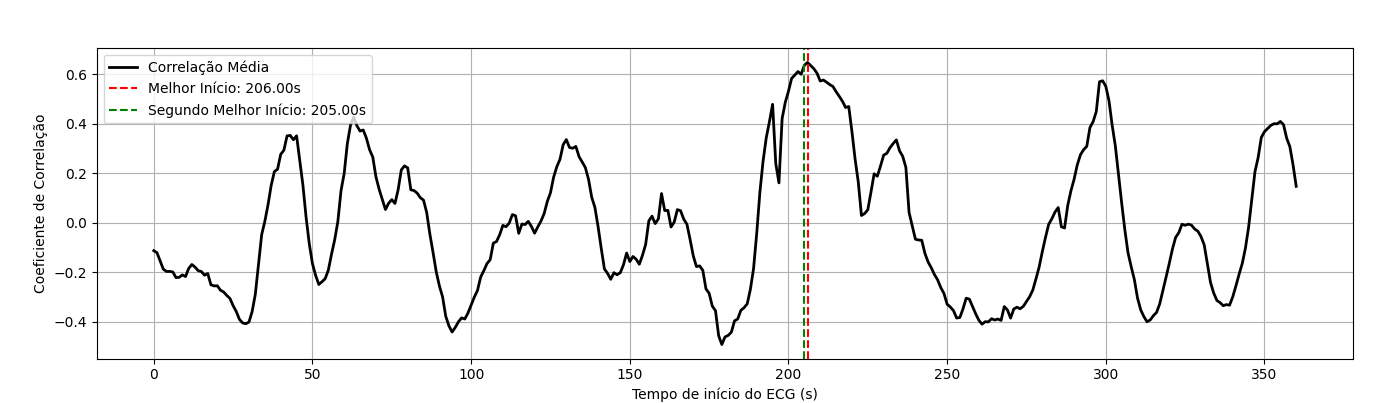
\includegraphics[width=\linewidth]{imagens/mean_corr_L9.png}
        \caption{Correlação média entre os valores de frequência cardíaca obtidos a partir do ECG de referência e os valores estimados pelos métodos de rPPG para o paciente 2}
        Fonte: autoria própria
        \label{fig:mean-corr-L9}
\end{figure}


Para o paciente 3, foi realizada a sincronização de forma similar à utilizada na coleta de validação, de forma que foi gerado um ruído no eletrocardiograma causado pela desconexão e reconexão de um dos eletrodos. Esse ruído insere um pico na forma de onda do ECG, conforme a \autoref{fig:ruido-ecg-L8}, sendo que considera-se o sinal no intervalo que se inicia 5 segundos após o momento respectivo a esse pico. Da mesma forma, o vídeo referente a esse paciente é cortado 5 segundos após o quadro em que se identifica a desconexão do eletrodo. 

\begin{figure}[h!]
    \centering
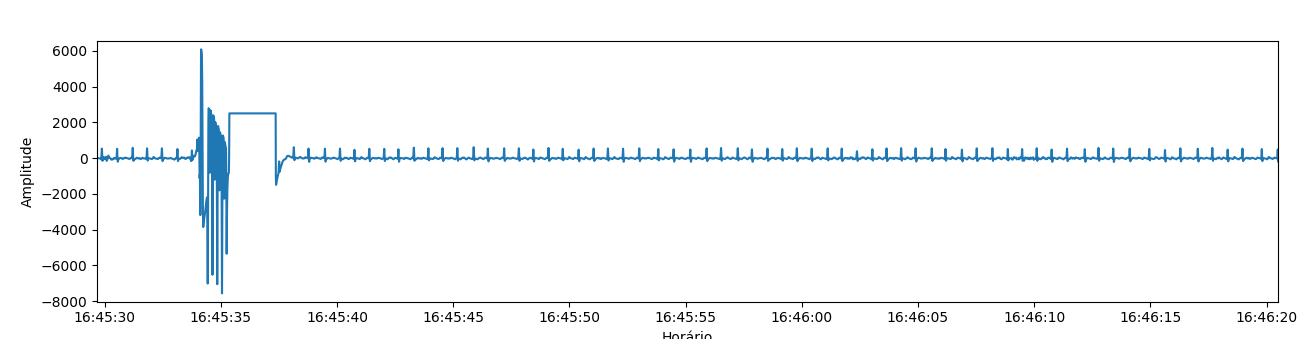
\includegraphics[width=1\linewidth]{imagens/ruido_ecg.png}
    \caption{Ruído gerado no eletrocardiograma do paciente 3 para sincronização dos dados de referência com o vídeo.}
    Fonte: autoria própria.
    \label{fig:ruido-ecg-L8}
\end{figure}

\subsection{Sinal de rPPG}

Os vídeos adquiridos em formato AVI foram utilizados para a extração dos sinais de pulso de volume sanguíneo por meio dos diferentes modelos e algoritmos supervisionados e não supervisionados de rPPG. A partir disso, a comparação da onda de fotopletismografia obtida remotamente com a onda de referência foi realizada por correlação cruzada, de forma a, primeiramente, sincronizar os dois sinais com base no atraso temporal que resulta no maior valor de correlação. Desse modo, foi calculada a correlação de Pearson entre os sinais sincronizados e os resultados para os pacientes 1 e 2 são apresentados na \autoref{tab:rppg_ppg_correlation}, em que os termos entre parênteses representam as bases de dados nas quais foram treinados cada modelo. 

\begin{table*}[h!]
\centering
\caption{Índices de correlação entre os sinais de rPPG e o sinal de PPG de referência para os pacientes 1 e 2.}
\resizebox{0.7\textwidth}{!}{
\begin{tabular}{llcc}
\hline
\textbf{Categoria} & \textbf{Método} & \textbf{Paciente 1} & \textbf{Paciente 2} \\
\hline

\multirow{7}{*}{Não supervisionado}
& CHROM & 0.0991 & 0.5754 \\
& GREEN & \textbf{0.3323} & 0.1350 \\
& ICA   & 0.1114 & 0.6783 \\
& LGI   & 0.1305 & 0.3575 \\
& OMIT  & 0.1336 & 0.3629 \\
& PBV   & 0.1252 & 0.5288 \\
& POS   & 0.1184 & \textbf{0.6884} \\

\hline

\multirow{10}{*}{Supervisionado}
& DeepPhys (PURE) & 0.1070 & 0.4276 \\
& DeepPhys (UBFC) & 0.1061 & 0.4992 \\
& EfficientPhys (PURE) & 0.0944 & 0.4576 \\
& EfficientPhys (UBFC) & 0.0949 & 0.4342 \\
& PhysFormer (PURE) & 0.0740 & 0.4547 \\
& PhysFormer (UBFC) & 0.0602 & 0.4141 \\
& PhysNet (UBFC) & 0.0636 & 0.3151 \\
& PhysNet (PURE) & 0.0425 & 0.4367 \\
& TSCAN (PURE) & 0.1309 & \textbf{0.5650} \\
& TSCAN (UBFC) & \textbf{0.1430} & 0.4505 \\

\hline
\end{tabular}
}
\label{tab:rppg_ppg_correlation}
\end{table*}

Os sinais de rPPG que resultaram no maior coeficiente de correlação entre os métodos supervisionados foram gerados pelo modelo TSCAN treinado no dataset UBFC-rPPG para o paciente 1 e pelo modelo TSCAN treinado no dataset PURE para o paciente 2. Os sinais obtidos por métodos não supervisionados, por sua vez, que resultaram no maior coeficiente de correlação foram obtidos pelo método GREEN para o paciente 1 e pelo método POS para o paciente 2, sendo que esses sinais em comparação com a referência são apresentados na \autoref{fig:corr-waves-examples}. Reitera-se que essa análise não foi realizada para o paciente 3 devido à ausência do sinal de PPG de referência durante a coleta de dados. 

\begin{figure}[h!]
    \centering

    \begin{subfigure}{0.9\linewidth}
        \centering
        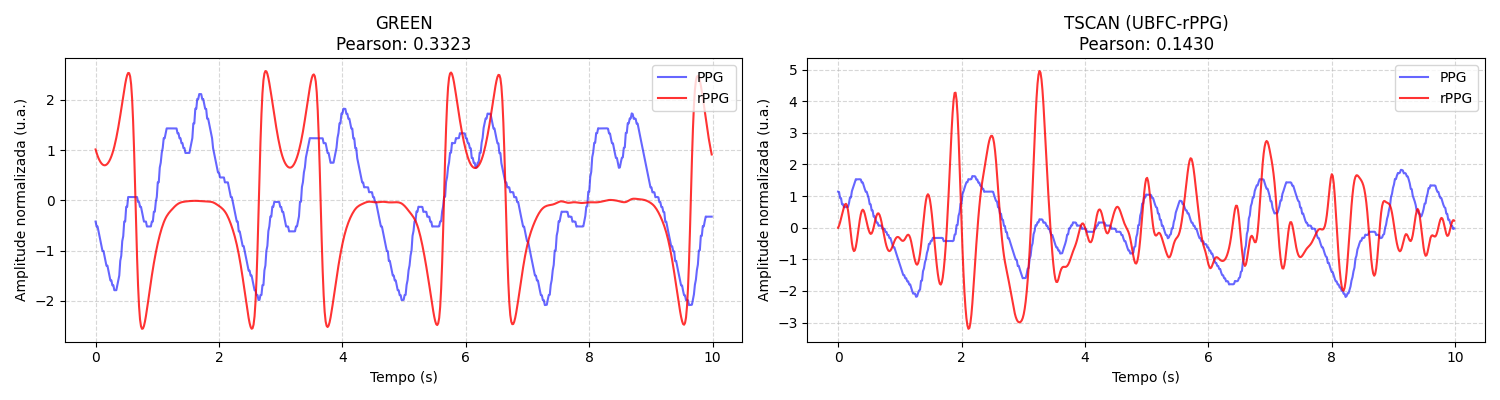
\includegraphics[width=\linewidth]{imagens/corr_examples_L7.png}
        \caption{Paciente 1}
        \label{fig:corr-waves-L7}
    \end{subfigure}

    \vspace{0.2cm}

    \begin{subfigure}{0.9\linewidth}
        \centering
        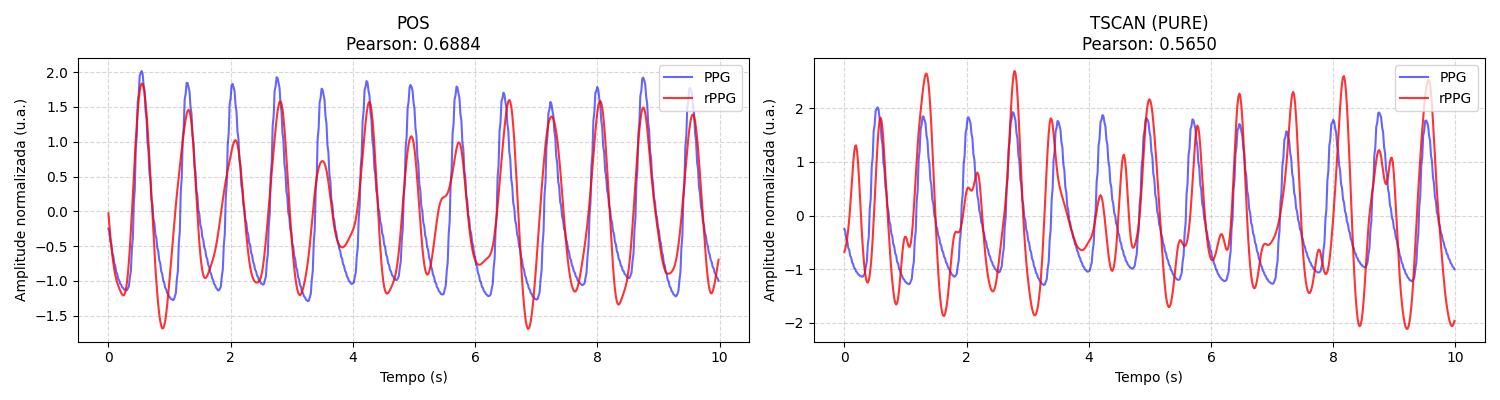
\includegraphics[width=\linewidth]{imagens/corr_examples_L9.png}
        \caption{Paciente 2}
        \label{fig:corr-waves-L9}
    \end{subfigure}

    \caption{Sinais de rPPG dos métodos que obtiveram o maior coeficiente de correlação de Pearson com o sinal de PPG de referência em cada paciente, considerando o alinhamento temporal realizado por meio de correlação cruzada.}
    Fonte: autoria própria.
    \label{fig:corr-waves-examples}

\end{figure}


\subsection{Estimativas de frequência cardíaca}

As estimativas de frequência cardíaca a partir dos sinais gerados por cada método de rPPG foram realizadas considerando o pico do espectro de potência obtido em janelas subsequentes de 15 segundos desses sinais. A partir disso, essas estimativas foram comparadas com as realizadas a partir do sinal de referência de ECG em janelas subsequentes de 15 segundos e foram calculados o erro médio absoluto e o erro médio quadrático em batimentos por minuto, assim como o erro médio percentual. Os resultados referentes aos pacientes 1, 2 e 3 são exibidos na \autoref{tab:rppg_ecg_metrics_all}.


\begin{table*}[htbp]
\centering
\caption{Métricas de erro da estimativa de frequência cardíaca por meio de cada método de rPPG em comparação com as realizadas a partir do ECG para os pacientes 1, 2 e 3.}
\resizebox{\textwidth}{!}{
\begin{tabular}{llcccccccccccc}
\hline
\textbf{Categoria} & \textbf{Método} 
& \multicolumn{4}{c}{\textbf{Paciente 1}} 
& \multicolumn{4}{c}{\textbf{Paciente 2}} 
& \multicolumn{4}{c}{\textbf{Paciente 3}} \\

\cline{3-14}

&
& MAE & RMSE & MAPE & SNR
& MAE & RMSE & MAPE & SNR
& MAE & RMSE & MAPE & SNR \\

\hline

\multirow{7}{*}{Não supervisionado}
& CHROM & \textbf{16.93} & \textbf{19.37} & \textbf{16.12} & -9.80 
& \textbf{0.89} & \textbf{1.06} & \textbf{1.15} & 0.14
& 3.65 & 6.34 & 4.22 & 0.07 \\

& GREEN & 25.89 & 26.13 & 24.75 & \textbf{-9.40}
& 11.60 & 14.99 & 14.93 & -8.39
& 24.60 & 27.50 & 27.02 & -10.80 \\

& ICA & 39.70 & 41.61 & 38.24 & -11.06
& \textbf{0.89} & \textbf{1.06} & \textbf{1.15} & 2.66
& 18.56 & 21.59 & 20.30 & -7.68 \\

& LGI & 26.31 & 26.50 & 25.15 & -9.52
& 4.06 & 5.49 & 5.20 & -3.92
& \textbf{2.59} & \textbf{4.99} & \textbf{3.02} & -2.51 \\

& OMIT & 26.31 & 26.50 & 25.15 & -9.54
& 4.06 & 5.49 & 5.20 & -3.79
& 4.49 & 7.99 & 5.11 & -4.03 \\

& PBV & 26.31 & 26.50 & 25.15 & -9.53
& 1.29 & 1.51 & 1.67 & -0.45
& 2.80 & 5.05 & 3.25 & -1.41 \\

& POS & 28.82 & 34.73 & 27.83 & -9.74
& \textbf{0.89} & \textbf{1.06} & \textbf{1.15} & \textbf{2.83}
& \textbf{2.59} & \textbf{4.99} & \textbf{3.02} & \textbf{1.51} \\

\hline

\multirow{10}{*}{Supervisionado}
& PhysFormer (PURE) 
& \textbf{16.97} & \textbf{26.69} & \textbf{16.43} & \textbf{-6.07}
& 5.68 & 9.53 & 7.21 & -3.85
& 8.25 & 15.92 & 9.08 & -2.56 \\

& PhysFormer (UBFC) 
& 40.54 & 41.43 & 38.67 & -7.96
& 3.09 & 5.87 & 3.91 & -2.61
& 8.53 & 14.37 & 9.42 & -1.96 \\

& EfficientPhys (PURE) 
& 45.47 & 46.69 & 43.43 & -10.40
& 6.44 & 10.87 & 8.18 & -3.10
& 6.82 & 13.82 & 7.52 & \textbf{-0.87} \\

& EfficientPhys (UBFC) 
& 48.49 & 49.84 & 46.33 & -8.49
& 8.27 & 12.05 & 10.52 & -3.72
& 6.82 & 13.82 & 7.52 & -1.61 \\

& PhysNet (PURE) 
& 33.15 & 36.16 & 31.72 & -11.06
& 5.09 & 8.34 & 6.61 & -2.80
& \textbf{1.20} & \textbf{1.87} & \textbf{1.38} & -1.66 \\

& PhysNet (UBFC) 
& 26.20 & 29.30 & 25.10 & -8.59
& 7.78 & 11.48 & 9.89 & -6.01
& 17.86 & 23.15 & 19.59 & -5.36 \\

& TSCAN (PURE) 
& 50.16 & 53.07 & 47.87 & -8.56
& \textbf{1.42} & \textbf{2.05} & \textbf{1.82} & \textbf{-1.25}
& 17.62 & 24.35 & 19.47 & -4.96 \\

& TSCAN (UBFC) 
& 33.15 & 36.16 & 31.72 & -9.69
& 3.93 & 8.05 & 4.96 & -2.87
& 16.61 & 22.73 & 18.59 & -3.96 \\

& DeepPhys (PURE) 
& 51.00 & 51.35 & 48.77 & -11.68
& 13.56 & 19.26 & 17.37 & -3.50
& 29.52 & 34.72 & 32.99 & -6.25 \\

& DeepPhys (UBFC) 
& 50.16 & 51.83 & 47.81 & -10.24
& 10.79 & 16.05 & 13.74 & -2.71
& 18.72 & 25.62 & 21.06 & -3.07 \\

\hline
\end{tabular}
}
\label{tab:rppg_ecg_metrics_all}
\end{table*}

É possível observar que o método não supervisionado que resultou no menor valor de erro absoluto médio para o paciente 1 foi o método CHROM. Em relação ao sinal do paciente 2, os métodos CHROM, ICA e POS resultaram nos menores valores de erro comparados ao restante dos métodos. Além disso, os métodos LGI e POS foram os que resultaram nos menores valores de erro para as estimativas de frequência cardíaca a partir dos sinais do paciente 3. No que se refere aos métodos supervisionados, por sua vez, o modelo PhysFormer treinado do dataset PURE foi o que apresentou o melhor resultado para o paciente 1, o modelo TSCAN treinado no dataset PURE resultou no menor valor de erro para as estimativas do paciente 2 e o modelo PhysNet treinado no mesmo dataset foi o que obteve o melhor resultado para o paciente 3. À parte isso, a comparação entre todos os métodos permite analisar que o método POS foi o que resultou na melhor relação sinal-ruído para os sinais dos pacientes 2 e 3. Já para o paciente 1, o sinal gerado pelo modelo PhysFormer treinado na base de dados PURE foi o que apresentou o melhor valor para essa métrica.

Observa-se, por fim, que os métodos CHROM, ICA e POS aplicados ao sinal do paciente 2 resultaram no menor valor de erro absoluto médio entre todos os algoritmos não supervisionados. Da mesma forma, o modelo TSCAN treinado no dataset PURE também aplicado ao sinal do paciente 2 resultou no menor erro absoluto médio entre os modelos supervisionados. Na \autoref{fig:best-specs-L9}, pode-se analisar os espectrogramas de dois desses sinais, a partir dos quais é possível identificar a região da frequência de maior densidade de potência de forma distinguível ao longo de toda a duração do sinal. 

\begin{figure}[h!]
    \centering
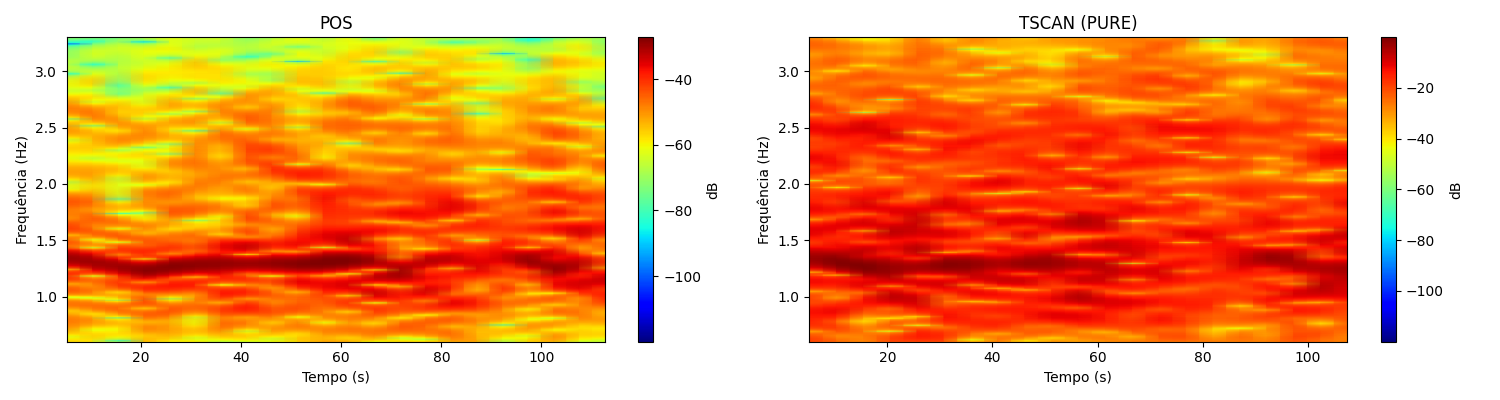
\includegraphics[width=1\linewidth]{imagens/best_specs_L9.png}
    \caption{Espectrogramas de dois dos sinais de rPPG cujas estimativas de frequência cardíaca resultaram no menor erro absoluto médio em relação às estimativas obtidas por meio do ECG.}
    Fonte: autoria própria
    \label{fig:best-specs-L9}
\end{figure}

Similarmente, os espectros de potência desses sinais apresentados na \autoref{fig:best-psd-L9} permitem a identificação do pico referente à essa frequência, a partir da qual pode ser realizada a estimativa do valor de frequência cardíaca. Nesse caso, a análise em frequência foi realizada no sinal completo com duração próxima a dois minutos. Em comparação, as estimativas de frequência cardíaca por janela são apresentadas na \autoref{fig:best-estimates-L9}. 


\begin{figure}[h!]
    \centering
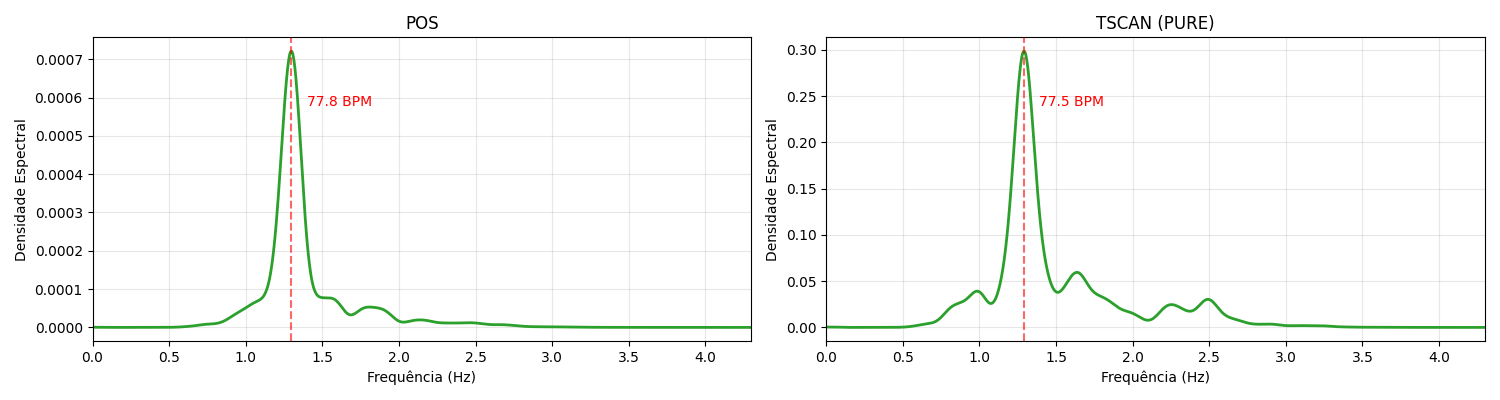
\includegraphics[width=1\linewidth]{imagens/best_psds_L9.png}
    \caption{Espectros de potência de dois dos sinais de rPPG cujas estimativas de frequência cardíaca resultaram no menor erro absoluto médio em relação às estimativas obtidas por meio do ECG}
    Fonte: autoria própria
    \label{fig:best-psd-L9}
\end{figure}

\begin{figure}[h!]
    \centering
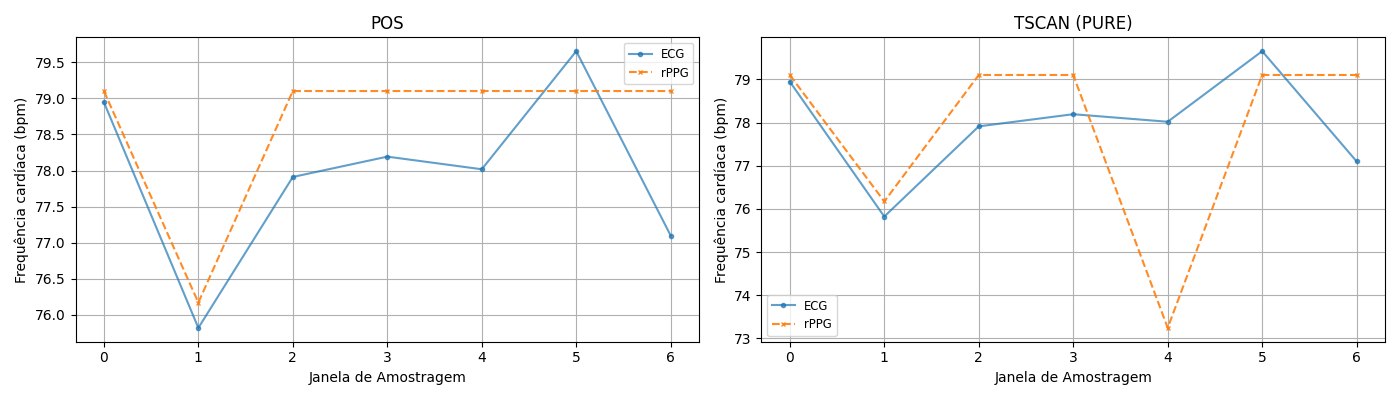
\includegraphics[width=1\linewidth]{imagens/best_estimates_L9.png}
    \caption{Estimativas de frequência cardíaca por janela obtidas por meio de dois dos métodos de rPPG que resultaram no menor erro absoluto médio em relação às estimativas obtidas por meio do ECG}
    Fonte: autoria própria
    \label{fig:best-estimates-L9}
\end{figure}

Ademais, é possível observar o erro absoluto médio entre todos os métodos não supervisionados em comparação com os métodos supervisionados em cada janela para os pacientes 1 e 2 na \autoref{fig:mean-error-per-window-preliminar}. Verifica-se que, para cada paciente, os dois tipos de métodos possuem alguns picos de erro em comum, a exemplo da janela 5 do sinal do paciente 2, que representa o maior erro para ambos os tipos de algoritmo. De forma análoga, a janela de índice zero desse sinal é a que resulta no menor erro absoluto médio para os dois tipos de método.

\begin{figure}[h!]
    \centering
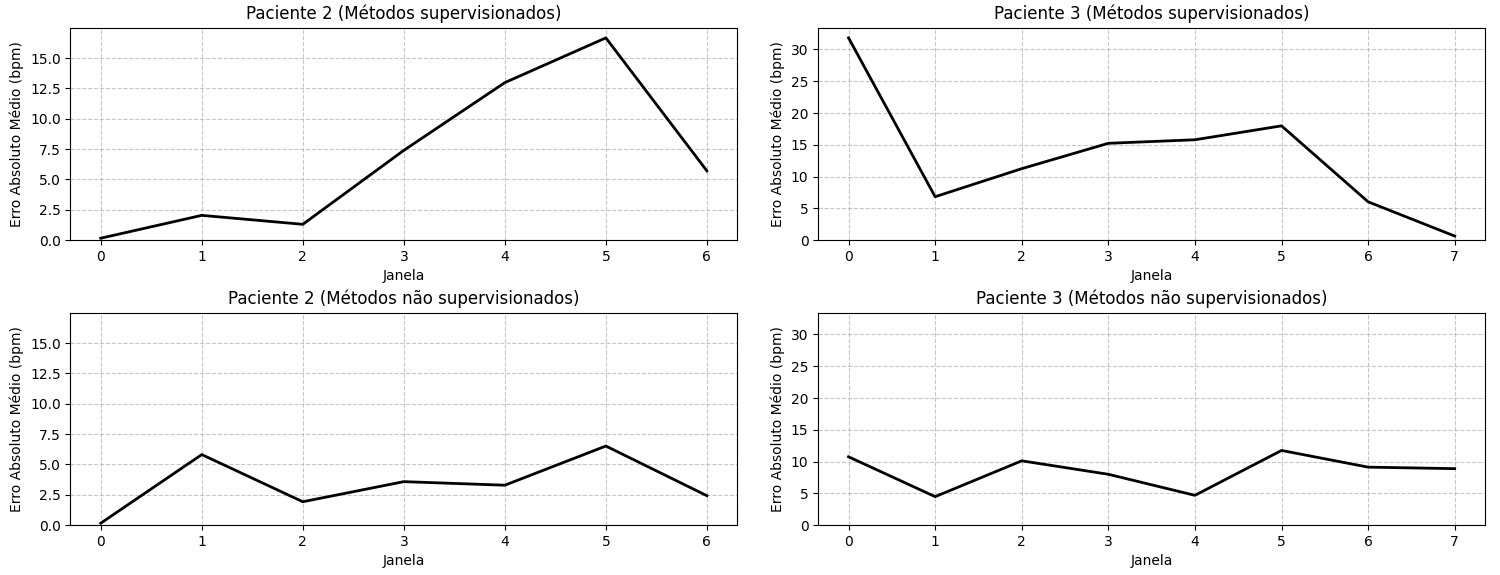
\includegraphics[width=1\linewidth]{imagens/mean_error_per_window_2e3.png}
    \caption{Erro absoluto médio por janela das estimativas de frequência cardíaca realizadas a partir dos métodos supervisionados e não supervisionados para os pacientes 2 e 3.}
    Fonte: autoria própria
    \label{fig:mean-error-per-window-preliminar}
\end{figure}


% \clearpage
\section{Coleta de validação}

Na coleta de validação, foram extraídos dois vídeos de um indivíduo saudável e os sinais de eletrocardiograma correspondentes. No primeiro vídeo coletado, o indivíduo apresentou pouca movimentação, enquanto no vídeo subsequente houve maior movimentação do rosto causada por fala, riso e rotações sutis da cabeça.

\subsection{Sincronização dos dados}

A sincronização entre os dados de vídeo e o sinal de referência foi realizada por meio da geração de um ruído no ECG devido a um impacto no eletrodo utilizado. Esse impacto é visível no sinal, conforme demonstra a \autoref{fig:ruido-ecg-valid}, sendo que foi considerado o sinal 5 segundos após o pico observado. Da mesma forma, são considerados os quadros do vídeo a partir de 5 segundos após o primeiro quadro em que é identificada a interferência no eletrodo.

\begin{figure}[h!]
    \centering
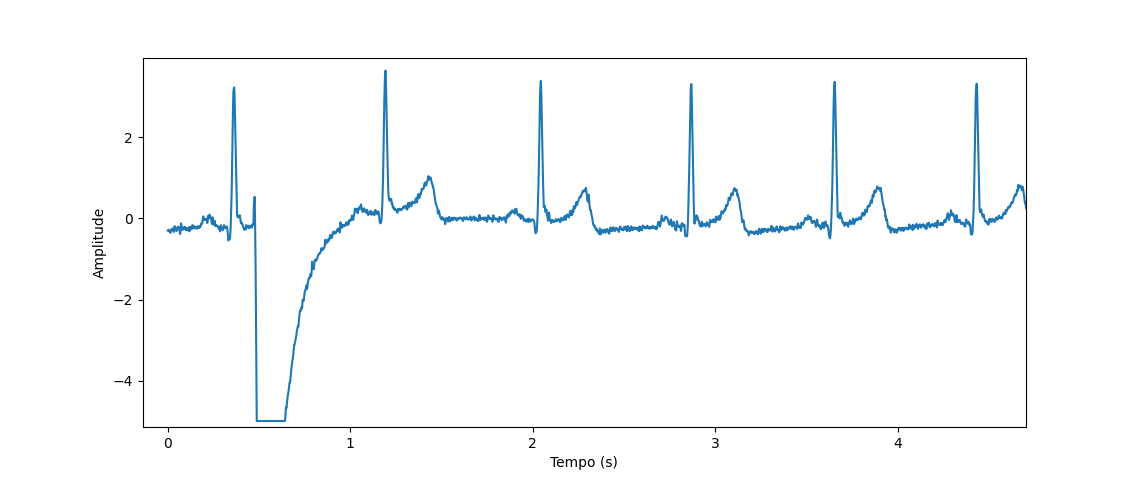
\includegraphics[width=0.7\linewidth]{imagens/ruido_ecg_valid.png}
    \caption{Exemplo do ruído gerado no eletrocardiograma para sincronização de dados da coleta de validação}
    Fonte: autoria própria
    \label{fig:ruido-ecg-valid}
\end{figure}

\subsection{Estimativas de frequência cardíaca}

% \begin{figure}[h!]
%     \centering
% 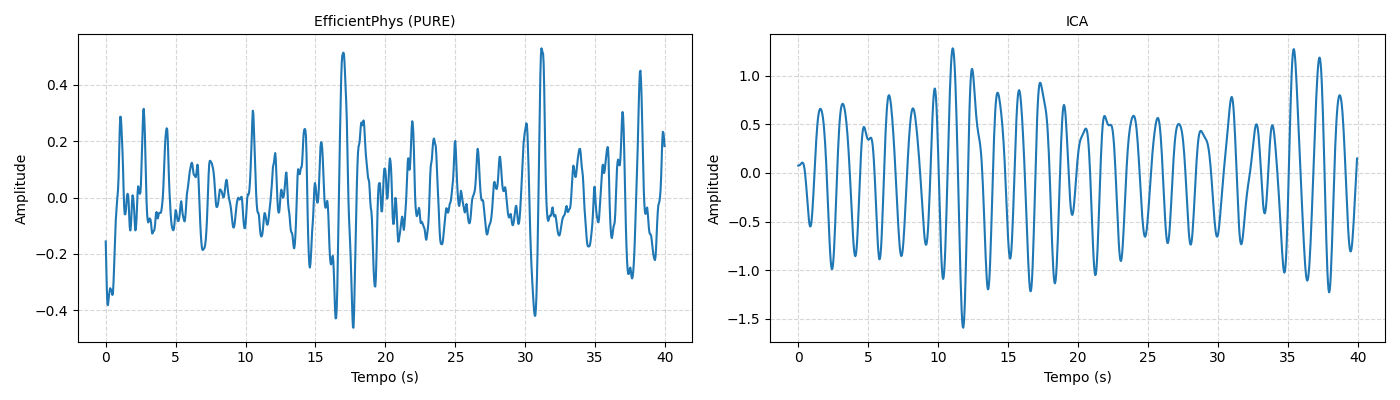
\includegraphics[width=1\linewidth]{imagens/waves_examples.png}
%     \caption{Exemplos de sinais resultantes extraídos a partir do primeiro vídeo da coleta de validação}
%     Fonte: autoria própria
%     \label{fig:waves-valid}
% \end{figure}

A partir dos sinais de pulso de volume sanguíneo obtidos por meio de cada um dos métodos e modelos de fotopletismografia remota aplicados aos dois vídeos adquiridos durante a coleta de validação, foram realizadas as estimativas de frequência cardíaca por meio da análise espectral desses sinais baseada na Transformada Rápida de Fourier em janelas subsequentes de 15 segundos. Essas estimativas foram comparadas com as obtidas a partir do ECG também em janelas subsequentes de 15 segundos. Os resultados dessas comparações são dispostos na \autoref{tab:rppg_ecg_metrics_valid}. 

\begin{table*}[h!]
\centering
\caption{Métricas de erro das estimativas de frequência cardíaca por meio de cada método de rPPG em comparação com as realizadas a partir do ECG para os vídeos 1 e 2.}
\resizebox{\textwidth}{!}{
\begin{tabular}{llcccccccc}
\hline
\textbf{Categoria} & \textbf{Método} 
& \multicolumn{4}{c}{\textbf{Vídeo 1}} 
& \multicolumn{4}{c}{\textbf{Vídeo 2}} \\
\cline{3-6} \cline{7-10}
& 
& \textbf{MAE} & \textbf{RMSE} & \textbf{MAPE} & \textbf{SNR} 
& \textbf{MAE} & \textbf{RMSE} & \textbf{MAPE} & \textbf{SNR} \\
\hline

\multirow{7}{*}{Não supervisionado}
& CHROM & 3.11 & 4.67 & 4.23 & 0.71 
         & 7.30 & 8.42 & 9.05 & \textbf{-5.40} \\

& GREEN & 8.85 & 11.73 & 12.18 & -6.40 
         & 7.59 & 9.03 & 9.71 & -8.42 \\

& ICA   & \textbf{1.69} & \textbf{2.25} & \textbf{2.32} & \textbf{4.74} 
         & 10.94 & 12.55 & 13.81 & -7.06 \\

& LGI   & 1.86 & 2.35 & 2.56 & 0.39 
         & \textbf{5.86} & \textbf{7.39} & \textbf{7.40} & -6.81 \\

& OMIT  & 1.86 & 2.35 & 2.56 & 0.21 
         & \textbf{5.86} & \textbf{7.39} & \textbf{7.40} & -6.75 \\

& PBV   & 2.03 & 2.46 & 2.79 & -2.44 
         & 6.98 & 7.74 & 8.63 & -7.94 \\

& POS   & 1.86 & 2.35 & 2.56 & 1.49 
         & 9.97 & 12.77 & 12.52 & -5.84 \\

\hline

\multirow{10}{*}{Supervisionado}

& PhysFormer (PURE) & 2.34 & 3.43 & 3.23 & -3.66 
                     & 12.67 & 16.13 & 15.56 & \textbf{-5.62} \\

& PhysFormer (UBFC) & 57.39 & 59.45 & 79.59 & -5.64 
                     & 32.36 & 36.73 & 41.80 & -7.68 \\

& EfficientPhys (PURE) & \textbf{1.69} & \textbf{2.25} & \textbf{2.32} & \textbf{-0.96} 
                        & \textbf{10.40} & \textbf{12.81} & \textbf{12.68} & -7.59 \\

& EfficientPhys (UBFC) & 5.58 & 8.14 & 7.71 & -2.99 
                       & 11.58 & 14.86 & 14.16 & -6.23 \\

& PhysNet (PURE) & 5.08 & 9.01 & 7.00 & -2.33 
                  & 11.09 & 16.73 & 13.90 & -6.40 \\

& PhysNet (UBFC) & 40.79 & 43.55 & 56.31 & -8.38 
                  & 39.06 & 40.00 & 50.00 & -9.31 \\

& TSCAN (PURE) & 3.64 & 4.96 & 5.02 & -2.71 
                & 11.09 & 15.57 & 13.42 & -6.47 \\

& TSCAN (UBFC) & 13.29 & 20.32 & 18.13 & -6.05 
                & 24.31 & 26.52 & 30.95 & -7.56 \\

& DeepPhys (PURE) & 13.27 & 16.11 & 18.39 & -5.56 
                   & 18.68 & 20.76 & 23.77 & -7.10 \\

& DeepPhys (UBFC) & 9.49 & 11.02 & 13.01 & -6.09 
                   & 16.01 & 20.10 & 20.28 & -6.70 \\

\hline
\end{tabular}
}
\label{tab:rppg_ecg_metrics_valid}
\end{table*}


Pode-se verificar que, entre os métodos não supervisionados, o método ICA foi o que resultou em estimativas de frequência cardíaca com o menor erro 
médio absoluto para o vídeo 1 e os métodos LGI e OMIT resultaram no menor erro para o vídeo 2. Em relação aos modelos supervisionados, o modelo EfficientPhys 
treinado na base de dados PURE foi o que apresentou o menor erro médio absoluto em ambos os vídeos. Ademais, o método ICA foi o que resultou, entre todos os métodos, 
no melhor valor de SNR para o vídeo 1, enquanto o método CHROM foi o que gerou o melhor valor para o vídeo 2. 

Por fim, entre todos os métodos avaliados em ambos os vídeos, o método ICA e o modelo EfficientPhys treinado na base PURE aplicados ao sinal do vídeo 1 
foram os que apresentaram os menores valores de erro médio absoluto. Os espectrogramas referentes aos sinais resultantes desses algoritmos são apresentados 
na \autoref{fig:specs-valid}, bem como seus respectivos espectros de potência na \autoref{fig:best-psd-valid}. A partir das figuras, observa-se que a 
frequência com maior densidade de potência pode ser identificada de forma distinguível, a partir da qual pode ser realizada a estimativa de frequência cardíaca. 
Nesse caso, a análise espectral foi realizada no sinal em sua completude. Complementarmente, as estimativas de frequência cardíaca realizadas por janela são 
dispostas na \autoref{fig:best-estimates-valid}.

\begin{figure}[h!]
    \centering
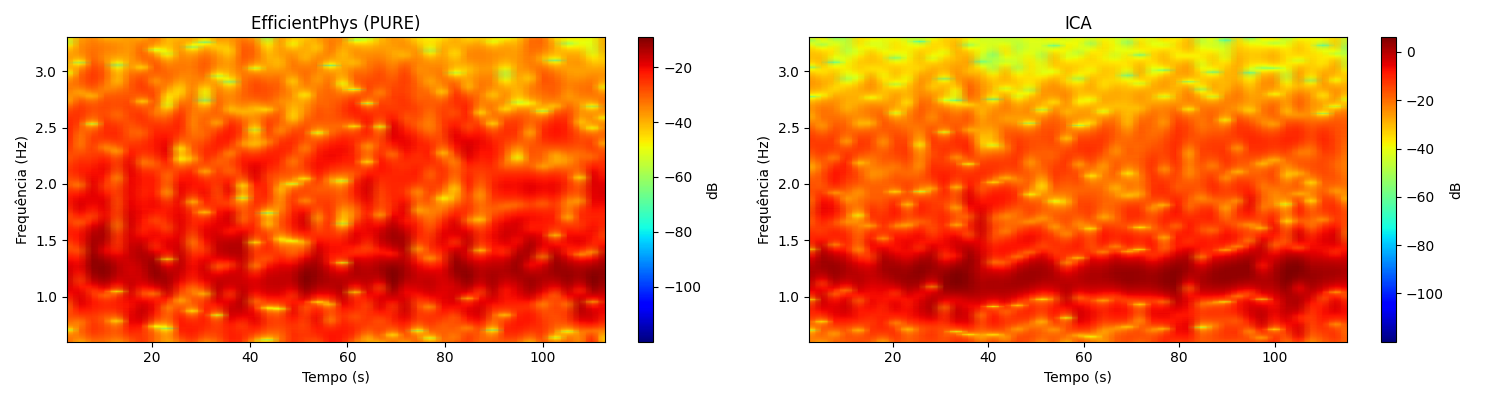
\includegraphics[width=1\linewidth]{imagens/best_specs_valid.png}
    \caption{Espectrogramas dos sinais cujas estimativas de frequência cardíaca resultaram no menor erro médio absoluto.}
    Fonte: autoria própria
    \label{fig:specs-valid}
\end{figure}

\begin{figure}[h!]
    \centering
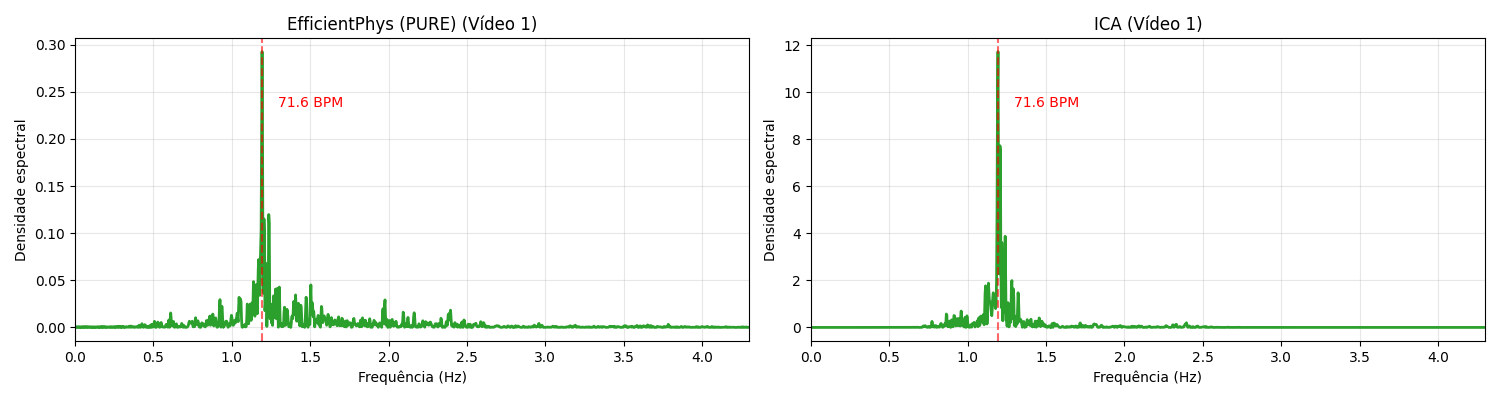
\includegraphics[width=1\linewidth]{imagens/best_psd_valid.png}
    \caption{Espectros de potência dos sinais cujas estimativas de frequência cardíaca resultaram no menor erro médio absoluto.}
    Fonte: autoria própria
    \label{fig:best-psd-valid}
\end{figure}

\begin{figure}[h!]
    \centering
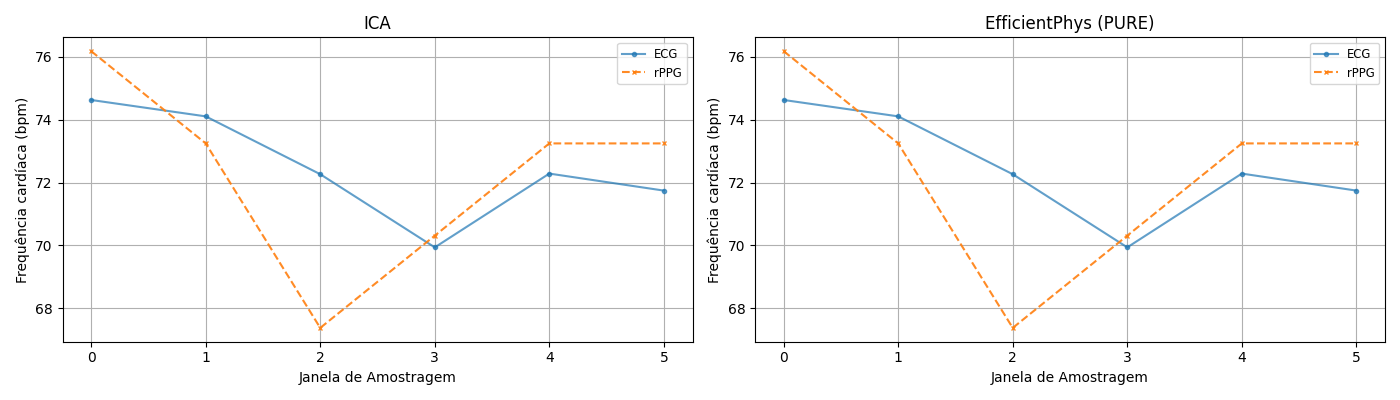
\includegraphics[width=1\linewidth]{imagens/best_estimates_valid.png}
    \caption{Estimativas de frequência cardíaca por janela dos sinais que resultaram no menor erro médio absoluto.}
    Fonte: autoria própria
    \label{fig:best-estimates-valid}
\end{figure}

Ademais, são apresentadas as curvas de erro absoluto médio dos métodos não supervisionados em comparação com os métodos supervisionados para os dois vídeos na \autoref{fig:mean-error-window-valid}. Pode-se observar como essas curvas de erro exibem comportamentos temporalmente semelhantes entre os dois grupos de métodos, com ocorrências coincidentes de aumento e redução do erro em múltiplas janelas consecutivas.

\begin{figure}[h!]
    \centering
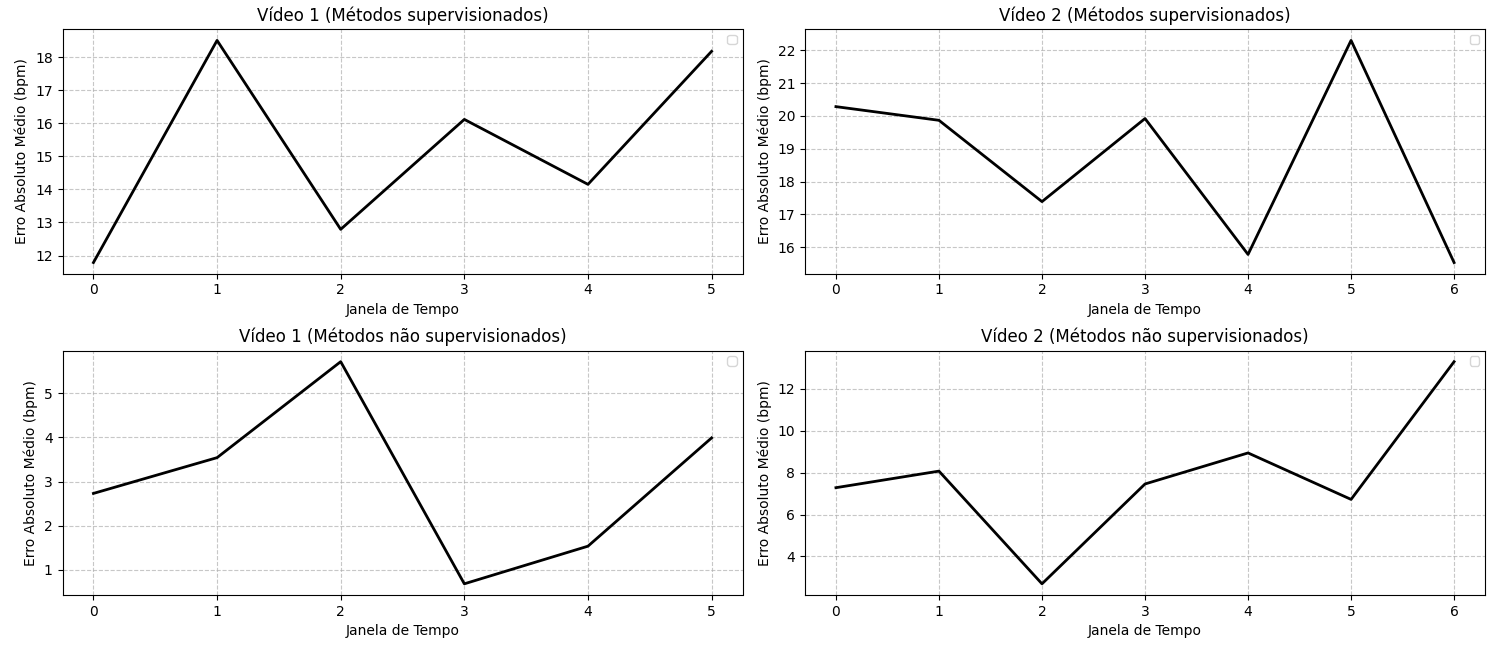
\includegraphics[width=1\linewidth]{imagens/mean_error_per_window_valid.png}
    \caption{Erro absoluto médio por janela dos métodos supervisionados e não supervisionados de cada vídeo da coleta de validação.}
    Fonte: autoria própria
    \label{fig:mean-error-window-valid}
\end{figure}
